\section{Logstash}
\subsection{Passage interbloc}
\label{subsec:passageinterbloc}
Au niveau du code, le passage d'une phase (bloc) à l'autre est implémenté via les \emph{SizedQueue} 
de ruby. Elles sont dimensionnées pour contenir 20 événements\footnote{appelés messages 
lorsqu'on parle de files de messages (queues en anglais), on parle bien ici 
des \textbf{événements} Logstash}. Ce paramètre n'est pas modifiable sans altérer 
le code source. Ces files ne sont pas conçues pour stocker des données à long terme. 

Ce choix technique (pour des raisons de performances), justifie l'utilisation d'un 
\textit{buffer}, comme \emph{Redis}.

\begin{figure}[H]
\center
\textbf{Bloc input $\Rightarrow$ file IF $\Rightarrow$ Bloc filtre $\Rightarrow$  file FO $\Rightarrow$ Bloc output}\\
\end{figure}
{\footnotesize Le bloc filtre est optionnel, dans ce cas là, il n'y a qu'une seule file.}

\subsection{Tolérance de pannes}
Les logs sont \textbf{importants}, les traiter efficacement est la raison d'être 
de Logstash. Il serait dommage d'en perdre à cause d'une défaillance quelconque 
rendant la destination indisponible\footnote{disque dur plein, problème réseau\ldots}.
%cf pipeline.rb et base.rb dans github

Tout d'abord : lors d'une indisponibilité, la plupart des plugins d'outputs tentent 
de renvoyer les événements vers leur destination. 
Tant que le transfert de l'évènement échoue, le bloc arrête de lire sa file d'attente
causant ainsi son remplissage\footnote{dans le cas où le bloc output dispose de  
multiples plugins, il existe des mécanismes pour pouvoir continuer à traiter les 
sorties saines mais cela impacte les performances}.

Par effet domino, la file \textit{filtre => output} se remplit jusqu'à ce que le 
bloc filtre ne puisse plus envoyer de nouveaux messages à cette file. 

Les plugins du bloc filtre vont également retenter d'envoyer ses messages, mais tant
que le problème ne sera pas débloqué en aval le bloc filtre va lui aussi 
refuser de lire les nouveaux messages arrivant dans la file \textit{input => filtre}.

Si cette dernière venait également à se remplir c'est le bloc input qui refuserait
de lire de nouveaux messages, provoquant l'indisponibilité de notre Logstash.
Dans le meilleur des mondes, les expéditeurs de données\footnote{chez nous syslog-ng} 
se comporteraient comme Logstash et attendraient patiemment que le problème se résolve 
en aval. Malheureusement cela n'est pas toujours possible (un switch n'a pas de place 
pour stocker ses logs) d'où l'importance d'un Redis afin de faire tampon.\footnote{Il 
existe d'autres outils que Redis, (dont ce n'est pas la fonction
principale) pour réaliser ce travail, ils sont plus adapté mais aussi moins documentés
dans leur utilisation avec Logstash.}

\subsection{Multithread}
\label{subsec:logstashmultithread}
{\footnotesize Attention ces informations sont pour le moment, \textit{(Jeudi 16 
Avril 2015)}, correctes mais sont amenées à changer, notamment concernant les outputs.}

Chaque plugin input utilise un thread. Cela permet d'éviter les engorgements si  
certaines entrées sont plus longues à traiter que d'autres.

Le bloc filtre entier utilise, par défaut, un seul thread. Mais, il est possible 
d'augmenter le nombre de threads affectés au traitement des filtres avec le \gls{flag}
-w lors du démarrage de Logstash.

À l'heure actuelle, le bloc output de logstash ne peut utiliser qu'un seul thread.
Il lit donc sa file de façon séquentielle. 
\subsection{Les codecs}
\label{subsec:logstashcodec}
Il existe également un \textit{pseudo-bloc} qui peut s'insérer dans les autres, ce 
bloc, \emph{codec} permet de gérer la \textit{représentation des données} c'est 
à dire qu'un codec est capable de lire ou d'écrire dans une syntaxe particulière 
comme par exemple collectd, ou, bien plus intéressant pour nous, netflow\footnote{Collecte d'information sur flux IP }. Pour simplifier c'est une sorte de plugin traduisant les évènements dans un format particulier ou depuis un format particulier, par exemple JSON.

\subsection{Moteur d'expression régulière}
\label{subsec:logstashregexengine}
Les expressions régulières utilisées par Logstash dans le plugin grok utilisent le 
moteur Oniguruma dont les spécifications sont disponibles à cette 
\href{http://www.geocities.jp/kosako3/oniguruma/doc/RE.txt}{adresse}\footnote{http://www.geocities.jp/kosako3/oniguruma/doc/RE.txt, 
si des symboles \textbf{ \textyen} apparaissent vous avez probablement un problème d'UTF8 sur 
votre navigateur, ils correspondent à des \textbf{ \textbackslash}}.
Ruby n'utilise plus Oniguruma depuis la version 2.0 mais son fork Onigmo\footnote{
dixit Wikipédia https://en.wikipedia.org/wiki/Oniguruma}. Mais cette évolution ne
s'applique pas à Logstash puisque ce dernier est codé en Jruby.

\subsection{Capabilities}
\paragraph{}
\label{subsec:logstashcapabilities}
\textbf{cap\_net\_bind\_service} permet à un utilisateur non privilégié (non root) 
d'écouter sur les ports privilégiés.

Les informations concernants les autres capabilities existantes sont disponibles dans
la page de manuel correspondante : \emph{man capabilities}.

\textbf{=+epi} signifie que l'on ajoute une \emph{capapbility} à un fichier. Plus 
précisement \textbf{=+} signifie que l'on écrase les droits précédents pour les remplacer
par les nouveaux. \textbf{e, p} et \textbf{i} sont la gradation de droits que l'on peut 
attribuer à un fichier avec les capabilities\footnote{\scriptsize{https://www.kernel.org/pub/linux/libs/security/linux-privs/kernel-2.2/capfaq-0.2.txt}}.
\begin{itemize}
    \item \textbf{effective}: indique si la capability est utilisée actuellement
    \item \textbf{permited}: définit quelles capabilities sont autorisées pour un 
    processus donné
    \item \textbf{inherited}: permet de transmettre la capability à un autre programme
\end{itemize}
\textbf{Note}: par défaut, changer le propriétaire d'un fichier de root, à non root enlève
les capabilities associées à ce dernier\footnote{\scriptsize{http://stackoverflow.com/questions/17743062/changing-user-ids-for-assigning-additional-capabilities}}.

Pour vérifier les \textit{capabilities} d'un binaire, on utilise la commande 
\emph{getcap}.

\begin{lstlisting}[style=code,label={lst:getcapabilities}]
    getcap /bin/ping
    /bin/ping = cap_net_raw+ep
\end{lstlisting}

Pour enlever les capabilities, il faut utiliser la commande suivante.
\begin{lstlisting}[style=code,label={lst:unsetcapabilities}]
setcap cap_net_bind_service=-epi /usr/lib/jvm/java-1.7.0-openjdk-amd64/jre/bin/java
\end{lstlisting}

Enfin, il est possible de donner à un utilisateur non root, l'autorisation
de modifier certaines capabilities. Pour ce faire, il faut modifier le fichier \\[1mm]
\ipath{/etc/security/capability.conf}.

\section{Elasticsearch}
\subsection{Cluster ElasticSearch}
\label{subsec:elasticcluster}

La santé de notre cluster est maintenant considérée comme bonne, il peut supporter 
une panne.

Nous allons maintenant rajouter encore un node et ainsi répartir mieux la charge

\begin{figure}[H]
\center
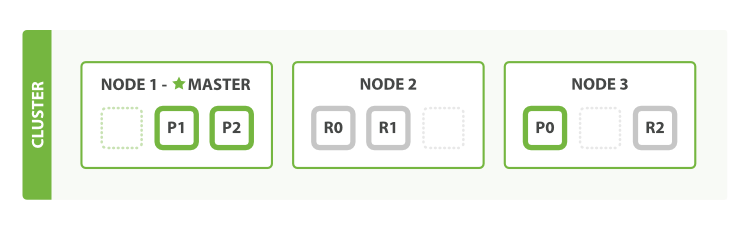
\includegraphics[width=1\textwidth]{elasticsearch/clustershard3.png}
\label{fig:clustershard3}
\caption{Cluster, 3 node, 1 index}
\end{figure}

Cette configuration fonctionne plus efficacement que la précédente puisqu'elle a 
accès à plus de ressource et que Elasticsearch répartie intelligemment ses ressources
et donc la charge de travail sur les différents nodes.

Remarque, si l'on perdait un node maintenant, nous nous retrouverions dans la configuration
numéro 2 (avec le failover), quitte à devoir réélir un master node. Notre état de santé,
serait toujours bon.

Pour voir des choses plus intéressantes, nous allons ajouter un shard répliqué (donc 3).

\begin{figure}[H]
\center
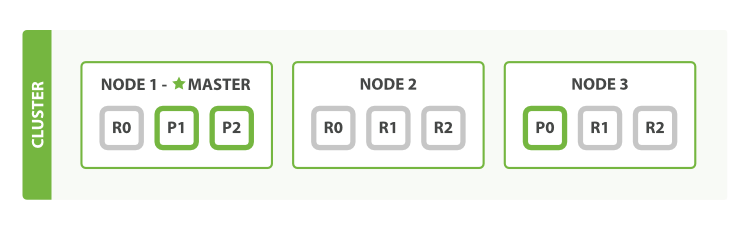
\includegraphics[width=1\textwidth]{elasticsearch/clustershard4.png}
\label{fig:clustershard4}
\caption{Cluster, 3 node, 1 index, mais plus de shards répliqués!}
\end{figure}


Les shards se répartissent de manière assez intuitivent.

Mais si nous enlevons le node 1\ldots

\begin{figure}[H]
\center
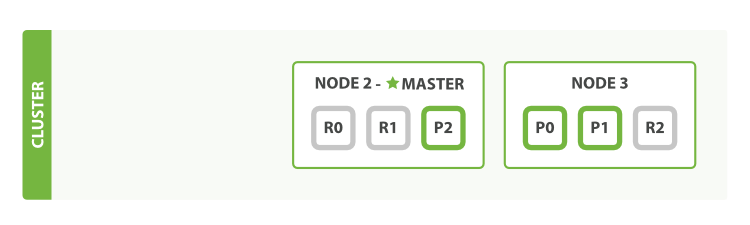
\includegraphics[width=1\textwidth]{elasticsearch/clustershard5.png}
\label{fig:clustershard5}
\caption{Cluster, 2 node, 1 index encore\ldots ou pas}
\end{figure}

Au moment précis de la coupure notre cluster est passé en mauvaise santé, car il 
n'avait plus de node master, et surtout des shards primaire étaient manquants.

Si une recherche avait été effectuée sur cet index à ce moment précis, des résultats partiels
auraient été obtenus, ainsi qu'un avertissement du fait que toutes les données n'étaient
pas disponibles.

On constate qu'une élection de master node a eu lieu. En constatant que deux shards 
primaires sont manquant il a immédiatement promu les shards répliqués au rang de 
shard primaires.

La santé de notre cluster est maintenant considérée comme moyenne, puisque tous ses
shards répliqués ne peuvent pas être affectés.



\subsection{Sense}
\label{subsec:elasticsense}
Ce module chrome a été développé par Boaz Leskes. Il sert de client à ElasticSearch
pour éviter d'avoir à le manipuler directement via curl.

Le développement (public) de ce module est arrêté depuis son intégration dans \emph{Marvel} 
le logiciel de monitoring et d'optimisation, vendu\footnote{voir basde page : 
\url{https://www.elastic.co/products/marvel/signup.html}} par la société \emph{elastic}.


\subsubsection{Installation}
Installer Sense est simple comme installer une extension 
Chrome\footnote{testé sur chromium} tierce.
Tout d'abord : récupérer le module à l'adresse \url{https://github.com/bleskes/sense}
en utilisant par exemple : 
\begin{lstlisting}[style=code,label=lst:gitclonesense]
git clone https://github.com/bleskes/sense.git
\end{lstlisting}

Il suffit ensuite de l'activer dans chromium :\\ 
chrome://extension => Developer mode => Load unpacked extension.
\begin{figure}[H]
\center
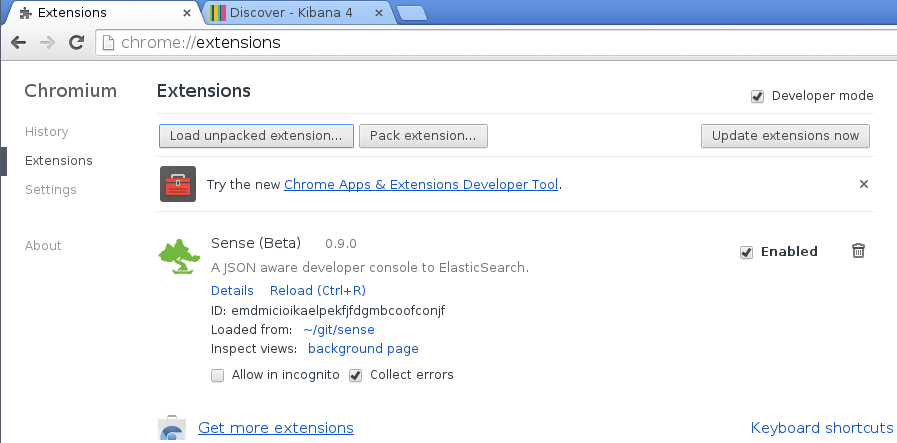
\includegraphics[width=12cm]{senseinstall.png}
\label{fig:senseinstall}
\caption{Plugin Sense installé dans chromium}
\end{figure}
Et voilà ! \footnotesize{(avec un accent anglais)}
\subsubsection{Utilisation de Sense}

\begin{figure}[H]
\center
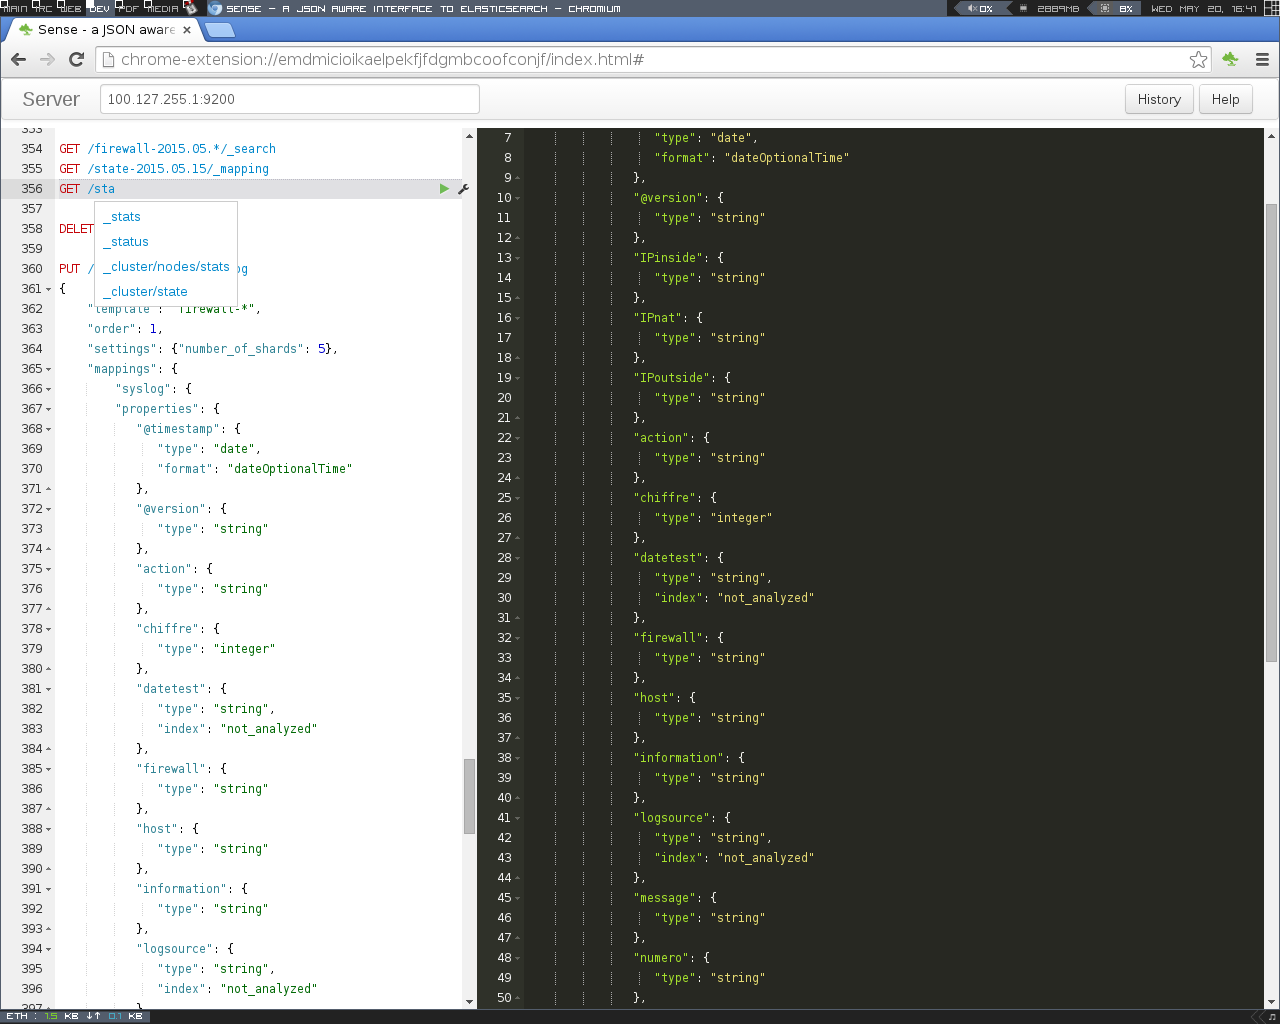
\includegraphics[width=1\textwidth]{sensegui.png}
\label{fig:sensegui}
\caption{Vue générale de Sense}
\end{figure}

Nous allons à l'aide de l'image ci-dessous brièvement expliquer le fonctionnement de Sense
\begin{figure}[H]
\center
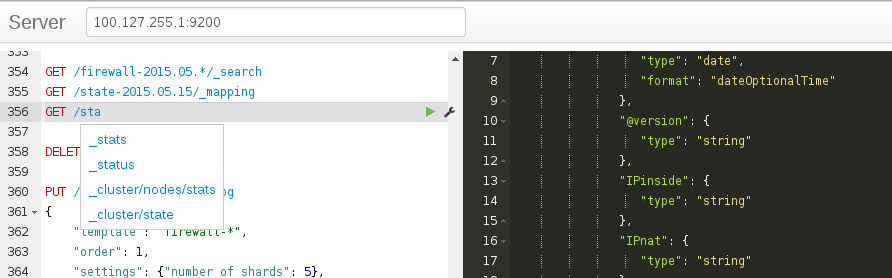
\includegraphics[width=15cm]{sensegui2.png}
\label{fig:sensegui2.png}
\caption{Zoom sur les fonctionnalités de Sense}
\end{figure}
Le formulaire \textbf{Server} situé en haut correspond à l'adresse et au port d'écoute 
de l'instance Elasticsearch sur laquelle on souhaite travailler.

Le panneau de gauche correspond au \textbf{panneau de requête}. On utilise l'API 
REST d'Elasticsearch pour envoyer des requêtes (recherches, modifications\ldots 
une présentation de l'API est réalisé précédemment). Il est à noté que le panneau 
de gauche est doté d'une autocomplétion pour les fonctions et les éléments standards 
d'Elasticsearch.

Le panneau de droite est le \textbf{panneau de réponse} aux requêtes. Les informations
nous parviennent en JSON.

\subsection{Full text}
\label{subsec:elasticfulltext}
%Le full text s'oppose aux valeurs exacts.
%Les champs dans lesquels on peut effectuer des recherches fulltext ont été au préalable 
%analysés (analyzed).
%Les champs non analysés sont traités comme des valeurs exacts.
%Certains types ne peuvent pas être analysé comme les chiffres, les booléens ou les dates.
%Il est possible de aussi possible de ne pas analyser une chaine de caractère.

Dans Elasticsearch la recherche full text désigne la recherche sur les champs analysés
(analyzed). Elle tire avantage du découpage (tokenisation) effectué au moment de 
l'indexation du champ.

Il faut tout d'abord bien comprendre que \textbf{"Le chien"} est différent de \textbf{"le chien"} 
ou encore de \textbf{"Lechien"}.

Il faut ensuite se rappeler la notion d'index et d'analyseur. L'analyseur va
décider de la façon dont les différents membres de la chaine de caractères vont être 
considérés. Après cette étape les membres vont être indexés et une recherche les 
renverra par popularité décroissante.

Puisqu'un exemple vaut mieux qu'un long discours, je vais m'inspirer de ceux donnés
dans \textit{"The Definitive guide to Elasticsearch"}.


Considérons 2 phrases :
\begin{itemize}
    \item The quick brown fox jumped over the lazy dog
    \item Quick brown foxes leap over lazy dogs in summer
\end{itemize}

\begin{figure}[H]
\center
\begin{tabular}{|l||c|c|}
\hline
\textbf{Termes}   & \textbf{P1}    & \textbf{P2}\\ \hline  
Quick   &       &  X\\ \hline  
The     &   X   &   \\ \hline
brown   &   X   &  X\\ \hline
dog     &   X   &   \\ \hline
dogs    &       &  X\\ \hline
fox     &   X   &   \\ \hline
foxes   &       &  X\\ \hline
in      &       &  X\\ \hline
jumped  &   X   &   \\ \hline
lazy    &   X   &  X\\ \hline
leap    &       &  X\\ \hline
over    &   X   &  X\\ \hline
quick   &   X   &   \\ \hline
summer  &       &  X\\ \hline
the     &   X   &  X\\ \hline 
\end{tabular}
\caption{Index des phrase}
\end{figure}
Lors d'une recherche full text, Elasticsearch va créer ce genre de listes.

Si je cherche \emph{quick brown}, le tableau ressemblerait à cela 


\begin{figure}[H]
\center
\begin{tabular}{|l||c|c|}
\hline
\textbf{Termes}   & \textbf{P1}    & \textbf{P2}\\ \hline  
brown   &   X   &  X\\ \hline
quick   &   X   &   \\ \hline \hline
Total   &   2   &  1 \\ \hline
\end{tabular}
\caption{Index correspondant à une recherche}
\end{figure}

On voit donc bien que la phrase la plus populaire est la phrase 1. On constate également
que Elasticsearch \emph{fait une différence entre \emph{Quick} et \emph{quick}}. 
Cela est est réglable (on peut, ne pas tenir compte de la casse).
Ce qu'il faut retenir c'est que pour discriminer efficacement, il est aussi possible
d'utiliser des syntaxe comme +fox, de même on peut faire une recherche avec un bloc
de deux termes pour être plus efficace : "over the" qui n'existe que dans P1.


\subsubsection{Recherches exactes}
Si dans notre mapping nous avons choisi de ne pas indexer certains champs (not\_analyzed)
ces champs ne seront pas cherchable en full text. Cela signifie que la valeur du 
champ devra correspondre exactement à celle de notre recherche. C'est notamment 
utile pour limiter le nombre de réponses.




\section{Kibana}
\subsection{Settings}
\label{subsec:settings}
Les paramètres de Kibana, concernent
uniquement Kibana, et pas Elasticsearch,\hyperref[fig:kibanatuto14]{ certaines informations} 
sont cependant affichées pour aider l'utilisation de Kibana mais il n'est pas possible 
de les modifier.

En revanche, il faut bien avouer que leurs consultations est plus agréable depuis 
Kibana que depuis l'export json d'Elasticsearch.

\begin{figure}[H]
\center
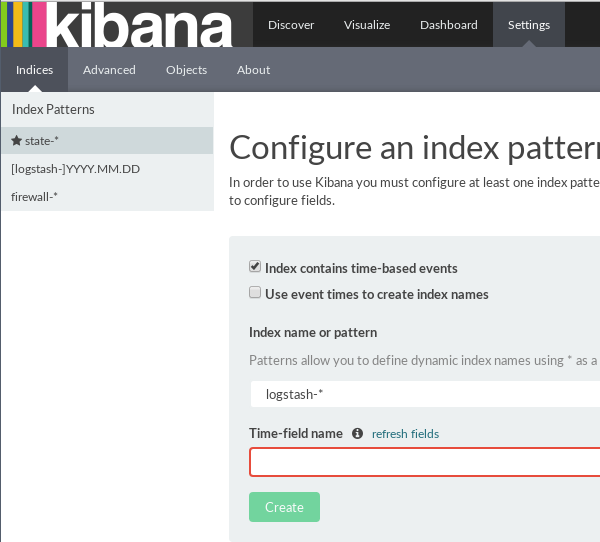
\includegraphics[width=1\textwidth]{kibanatuto/rap/20.png}
\label{fig:kibanatuto13}
\caption{Accueil de settings}
\end{figure}

Dans cette page vous pouvez créer de nouveaux ensembles d'index, ou en choisir un 
déjà existant.

En choisissant un index nous obtenons des informations sur son mapping, ce qui peut 
être utile pour effectuer des recherches plus pertinenentes.


\begin{figure}[H]
\center
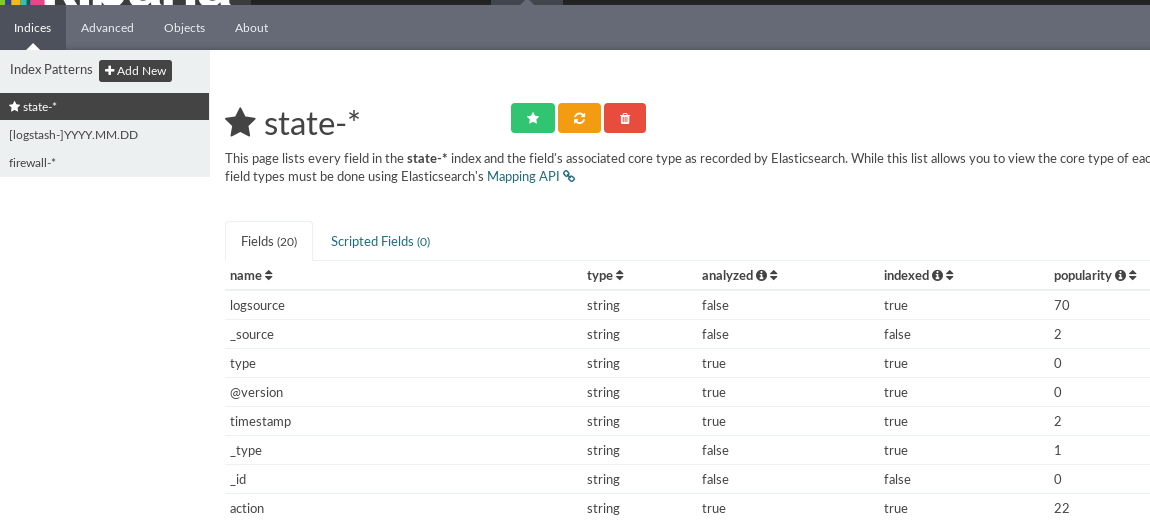
\includegraphics[width=1\textwidth]{kibanatuto/rap/22.png}
\label{fig:kibanatuto14}
\caption{Mapping d'un index}
\end{figure}

Enfin, c'est aussi dans cette section que l'on a une liste et que l'on peut supprimer les 
objets enregistrés (recherche, visualisations, dashboard)

\begin{figure}[H]
\center
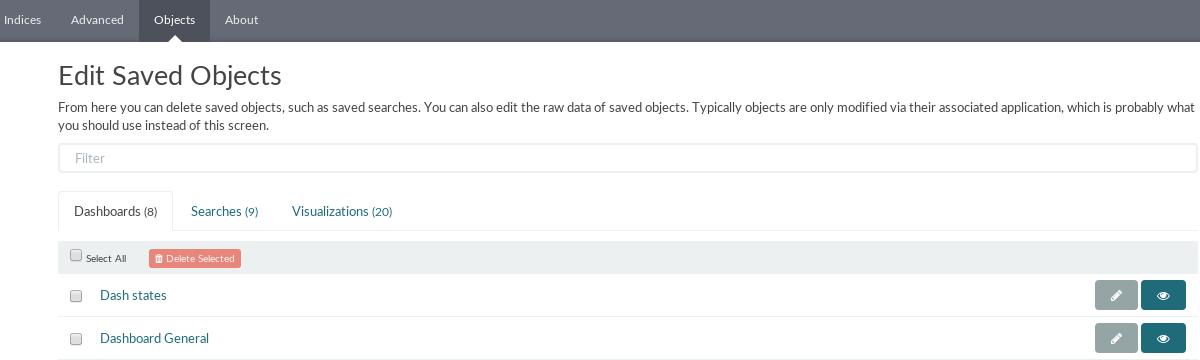
\includegraphics[width=1\textwidth]{kibanatuto/rap/23.png}
\label{fig:kibanatuto15}
\caption{Liste des objets}
\end{figure}

